% !TEX TS-program = pdflatex
% !TEX encoding = UTF-8 Unicode

% This is a simple template for a LaTeX document using the "article" class.
% See "book", "report", "letter" for other types of document.

\documentclass[11pt]{article} % use larger type; default would be 10pt

\usepackage[utf8]{inputenc} % set input encoding (not needed with XeLaTeX)

%%% Examples of Article customizations
% These packages are optional, depending whether you want the features they provide.
% See the LaTeX Companion or other references for full information.

%%% PAGE DIMENSIONS
\usepackage{geometry} % to change the page dimensions
\geometry{a4paper} % or letterpaper (US) or a5paper or....
% \geometry{margins=2in} % for example, change the margins to 2 inches all round
% \geometry{landscape} % set up the page for landscape
%   read geometry.pdf for detailed page layout information

%%% Line Spacing
\usepackage{setspace}
\onehalfspacing

\usepackage{graphicx} % support the \includegraphics command and options

% \usepackage[parfill]{parskip} % Activate to begin paragraphs with an empty line rather than an indent

%%% PACKAGES
\usepackage{booktabs} % for much better looking tables
\usepackage{array} % for better arrays (eg matrices) in maths
\usepackage{verbatim} % adds environment for commenting out blocks of text & for better verbatim
\usepackage{subfig} % make it possible to include more than one captioned figure/table in a single float
\usepackage{amsmath, amssymb, amsthm, lastpage}
% These packages are all incorporated in the memoir class to one degree or another...

%%% HEADERS & FOOTERS
\usepackage{fancyhdr} % This should be set AFTER setting up the page geometry
\pagestyle{fancy} % options: empty , plain , fancy
\renewcommand{\headrulewidth}{0pt} % customise the layout...
\lhead{Team \# 16677}\chead{}\rhead{Page \thepage\ of \pageref{LastPage}}
\lfoot{}\cfoot{\thepage}\rfoot{}

%%% SECTION TITLE APPEARANCE
%\usepackage{sectsty}
%\allsectionsfont{\sffamily\mdseries\upshape} % (See the fntguide.pdf for font help)
% (This matches ConTeXt defaults)

%%% ToC (table of contents) APPEARANCE
%\usepackage[nottoc,notlof,notlot]{tocbibind} % Put the bibliography in the ToC
%\usepackage[titles,subfigure]{tocloft} % Alter the style of the Table of Contents
%\renewcommand{\cftsecfont}{\rmfamily\mdseries\upshape}
%\renewcommand{\cftsecpagefont}{\rmfamily\mdseries\upshape} % No bold!

%%% END Article customizations

%%% The "real" document content comes below...
%\date{}

\begin{document}
\begin{titlepage}
    \vspace*{\fill}
    \begin{center}
      \Huge{Rapid Scheduling: A Constraint Satisfaction
        Approach to River Usage}\\[0.5cm]
      \Large{Team: 16677}\\[0.4cm]
      \today
    \end{center}
    \vspace*{\fill}
  \end{titlepage}
\newpage
\vspace*{\fill}
\tableofcontents
\vspace*{\fill}
\newpage

\section{Preliminaries}
\label{sec:prelims}
%Possibly include some comparisons of our model to existing research if any.

\subsection{Introduction}
\label{sec:intro}
Scheduling problems are a regular and common task for today's computers.
Asking secretaries or other individuals to devise a functioning arrangement
of times, places, and any other number of factors seems almost inhumane given
that the use of technology simplifies and expedites the process.  Applying
such technology to the task of scheduling rafters for a season poses unique
challenges and variables.  Park management literature tends to focus
on minimizing the ecological impact of visitors to a river,
not scheduling these visitors\cite{ColoradoRiverPaper}.  It is possible for
our model to address some parts of this approach
(\textbf{Section \ref{sec:extensions}}), but we are more interested in
maximum visitation.

Our aim is to determine the maximum number of individuals we may schedule
for trips along the Big Long River: such that no campsites may be shared
on a given night and we desire to have the most satisfied individuals possible.
That is, satisfaction is diminished when visitors come into contact with other
groups or are forced to travel further than they desire in a given day
(travelling at their own pace is important).  We approach the problem as
one of constraint satisfaction, a class of concepts from artificial intelligence.
Many scheduling problems may be approached with local search or even genetic
algorithms.  We, however, appreciate the elegance achieved when
rephrasing this as a constraint satisfaction problem.


\subsection{Definitions and Terminology}
\label{sec:defs}
% CSP a group of generally NP-hard problems.
% travel group
% itinerary
% NP-hard
% big O
% river length = L
% days in the season = S
% happiness as satisfaction: related to encounters and actual trip speed
% tolerance: brief description plus see section blah
% carrying capacity


\subsection{Assumptions and Simplifications}
\label{sec:assumptions}
% season length
% days traveled opposed to nights
% groups
% encounters
% happiness calculation as satisfaction (show equations)


\section{Details of the Model}
\label{sec:model-details}
Our model is structured as a constraint satisfaction problem solver.
The general definition
for such a problem is that - given variables ($X$), values ($D$),
and constraints ($C$) - find an assignment of value(s) in $D$
for each $X$ such that all constraints in $C$ are satisfied.
Good examples of this problem set are 2-SAT and coloring problems.

We view the problem of scheduling rafting trips as a progressive and dynamic
CSP: each day being a constraint satisfaction problem dependent upon the
solution to the previous day's problem.  By limiting the values any variable
may take on and applying efficient algorithms, the CSP becomes tractable and
we may successfully schedule river trips without the need of unreasonable
computing power.

\subsection{Constraint Satisfaction}
\label{sec:csp}
%variables, values, constraints (rules from problem statement)
%travel groups as variables
%campsites as values
%constraints

In general, our approach is to first consider that there are exponentially
many combinations of travel groups to campsites during their trip.  Many of
these combinations, however, are invalid given the constraint of no two
travel groups being allowed to stay at the same campsite.  This is perhaps
the greatest limiting factor in the problem as it applies to all campers
passing through the same territory on a given day.  This is an $n-ary$
constraint: the constraint relating $n$ variables.  Such constraints are
computationally challenging for many problems, but our problem space is limited
enough that the computations are relatively painless ($O(n^2)$ with $n$ as
number of travel groups) to pair all campers and detect collisions at any
campsite.  There were few other constraints involved in solving the problem
as we were mostly interested in solutions to our schedule.

As we have been discussing, each travel group was considered to be a variable
in the CSP and campsites were considered the values.  The domain of these
values (for each travel group) varied day to day depending upon the distance
each group was capable of travelling.  This travel distance was derived from
a group's average speed of 4 or 8 mph, $v$,  multiplied with a uniformly distributed
random variable for desired daily time spent on the water, $t$.  This variable is such
that the travel distance per day would allow the group to complete the trip
within the allotted time of 7-19 days. The following few equations explicitly
describe these relationships:
$$v*t=OptimalDayDistance$$
$$v*t*7\geq L$$
So in generating any travel group, we ensure the group is reasonably
parameterized for finishing a trip on time.  Each group is also randomly
assigned, uniformly distributed, a day for departure (dDay) such that
$$v*t*7+dDay\leq S$$
That is, a group's maximum travel speed will allow them to finish before
the close of the season.

Groups are generated en masse using a varitey of uniformly distributed
variables.  It is possible to load in a file containing group information
so that the program will work on problems of corporeal, rather than testing
and verification, import.  Once groups are generated and basic parameters
are set (discussed in \textbf{Section \ref{sec:high-params}}) the program begins
attempting to produce a solution through our CSP solver.

\subsubsection{Backtracking Search}
In order to solve a CSP, one must navigate the vast multitude of combinations
for variables and values. We utilize a backtracking search algorithm to
assign campsites to our travel groups on a daily basis.  On any given day
$d$, the solver looks to see which groups are set to depart on $d$ and
subsequently adds them to a list, $toDepart$.  All groups still on the
river from the previous day are added to $toDepart$, creating a list of all
travel groups requiring some movement for day $d$.  In order to determine
appropriate movements, the groups are assigned campsites (analagous to
distance traveled for the day) one-by-one.  Following
a pairing, the full day's assignment is checked to see if this pairing is
consistent with current progress.  If the pairing doesn't violate any other
existing pairings, it is added to the day's list of assignments.  We then
proceed to the next travel group.

Encountering failed pairings causes the algorithm to attempt another pairing
until success is achieved or failure must be returned.  If failure occurs,
the algorithm returns to the most recent pairing, undoes this pairing, and
then attempts a new pairing.  The entire process is structured as a
depth-first-search. When a day's assignment is complete, the algorithm creates
a new CSP for the next day and executes again, deepening the recursing into
another day.  \textbf{Figure~\ref{fig:searchExample}} highlights the major steps
involved in this process and provides a simple example.  The example is
simplified so that only two groups are being assigned a possibility of two
campsites.  The algorithm begins by assigning site $1$ to group $A$, denoted
by the diamond below and to the left of the tree-top.  Then assigning
site $1$ to $B$ is tried but found to fail, so the algorithm assigns site
$2$ to $B$ (rightmost circle).  At this point, a the day would ``end'' and
the algorithm would begin attempting to schedule the new day.  In the event
of a failure on a new day, the algorithm continues jumping up a level, as
seen in the example, even to the extent of needing to reschedule a previous
day.

\begin{figure}[h]
  \centering
  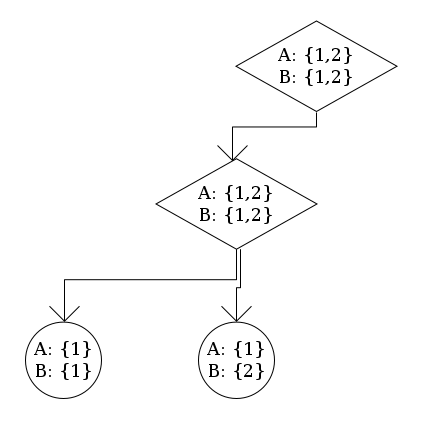
\includegraphics[scale=0.5]{imgs/searchExample.png}
  \caption{An example of the backtracking algorithm's attempt to schedule
    travel groups $A$ and $B$ with campsites $1$ and $2$.}
  \label{fig:searchExample}
\end{figure}

Our solver is optimized to attempt maximal satisfaction of the travelers.
That is, the possible campsites a group may travel to are presented to the
solver in order of ideal travel distance.  While not every group is guaranteed
to always travel their desired distance, the algorithm attempts to satisfy
this ``fuzzy constraint''.  We also calculate the number of encounters
between groups.  After the itineraries are created, each group's campsite
listing is checked to determine how many groups passed and were passed by
this specific group.  By combining the amount of erring from ideal travel distance
and encounters with other groups, we obtain the aforementioned effect on
satisfaction.  This effect is calculated post-solution.
Throughout the course of operation, the solver relies heavily on several
parameters to relax the problem and make solutions more attainable.

\subsection{Usage of High-Level Parameters}
\label{sec:high-params}
% group size
% river length (maybe)
% days in the season
% number of sites
Given some of the information in the prompt and our findings, as discussed
in \textbf{Sections \ref{sec:defs}} and \textbf{\ref{sec:assumptions}}, our program
is designed to adjust its operation depending on various conditions.  The
parameter of greatest variability, number of travel groups, effects how
many groups we generate at the beginning, the load distribution on portions
of the season, and some of the satisfaction scores for other groups. Varying
this value was crucial in analyzing the model, discussed in \textbf{Section
\ref{sec:results}}.

Values that tend to be static include the river length, number of days in
the season, and number of campsites.  While each of these is capable of
drastically effecting the outcome of any given attempt, the values have a
well-defined range (see \textbf{Section \ref{sec:assumptions}}).  The problem
could be generalized beyond these variables such that the CSP solver attempts
to find optimal values for these as well, but this would likely place our
problem into the realm of truly NP-hard problems.


\subsubsection{Tolerance}
Built into the algorithm is a $tolerance$ variable: designed to create a
range for the distance a travel group may cross in a given day.  This variable
is straightforward at the outset but provides several neat nuances for additional
complexity in the solution.  The introduction of a range to the CSP allows
for a larger domain of solutions and, therefore, variability.  In our case,
we desire such flexibility, to account for the real-world implications of
directing human beings.  Tolerance extends within the model as a sort of
aggregate for many of the various instances where we might expect variability
--- such as inclement weather, cancellations, or slow travel groups---,
without having to introduce variability into every aspect.  This may seem
like a stretch of the model's design, but any fuzziness for
any aspect introduces variability into the solutions.  We are satisfied that
tolerance is an opportunistic variable for allowing more groups to be
scheduled and thus for the rafting season to be enjoyed by more individuals.



\section{Predictions and Analysis}
% address all of our graphs
% address the question of how to mix the groups (i.e. oar versus motorized)


\subsection{General Expectations}
\label{sec:expectations}
Before creating the model we developed a few “common sense” expectations of
the results. For instance, it “makes sense” that increasing the group size
would make it harder to schedule each group at their desired time. The more
groups one is trying to schedule, the faster the schedule fills up. However,
as the number of groups on the river during a season increases, it would
become more and more likely that groups would pass each other. Passing
would even be mandatory if the groups are travelling at different daily
speeds; consider a group with a daily speed of 8 mph leaving a few days
after a group travelling at 4 mph.

We also expected that as the tolerance for which campsite groups stayed at
each night increased, so would the ease of scheduling each group. The
greater the tolerance, the greater the likelihood of finding a site to stay
at if other groups are also in the area. It also “made sense” to us, however,
that an increase in tolerance would cause a decrease in overall happiness.
An increase in tolerance would allow groups to travel less than or more
than their desired time each day. This would decrease their happiness.

It was expected that assigning more groups to motor boats (those that travel
at 8mph) would increase the success rate. Groups that travel faster would
spend fewer days on the river, freeing up space for other campers faster,
and allowing more groups to travel on the river each season. We also
predicted that seasons with more uniform group speeds (e.g. seasons where
all groups travel at 4mph, or where all groups travel at 8mph) would be
happier. This is because groups travelling at the same speed are less likely
to pass each other, or to want to stay at the same campsite on the same night.
The greater the variation in group speed, the more likely it is faster
groups would have to pass slower groups.

\subsection{Results}
\label{sec:results}
Generally speaking, the results of the model were in line with our
expectations. For seasons with a 2-site camping tolerance, the success rate
was seen to decrease as the number of groups increased. See sparkline 1 in
figure X at the bottom of this page.

The success rate was one-hundred percent up for seasons with 5, 50, and 100
groups. Once the number of groups per season increased past 100, the
success rate began decreasing at an increasing rate. The success rate
dropped from 100 percent to 91 percent between 100 and 300 campers, then
from 91 percent to 25 percent between 300 and 500 campers. For seasons with
more than 500 campers, the success rate leveled off, appearing to have an
asymptote just above zero percent. The success rate for a season with 600
groups was five percent.

Similarly, the average happiness of each of the groups decreased as the
number of groups increased. See figure X, sparkline 2 at the bottom of
this page. Once the number of groups per season increased past 100, the
happiness rate began decreasing at an increasing rate. The happiness dropped
from 97.9 percent to 89.4 percent between 100 and 300 campers, then from 89.4
percent to 24.5 percent between 300 and 500 campers. For seasons with more
than 500 campers, the happiness rate leveled off, appearing to have an
asymptote just above zero percent. The happiness for a season with 600 groups
was 4.9 percent.

For seasons with a  1-site tolerance, the effect of group size was seen to
increase. See sparkline 3 in figure X at the bottom of this page. Both the
success rate and happiness of groups began dropping with a group size of
only 50 people. The success rate dropped from 100 percent to 96 percent
when group sized increased from 5 to 50 groups per season. By just 250
groups, both the success rate and the happiness were zero percent.

The tolerance for which campsite groups stayed at each night had a positive
effect on success rate of the scheduler and happiness of the groups. See
sparkline 4, figure X, at the bottom of the previous page. For seasons with
200 groups, a tolerance of zero campsites had a success rate of 0 percent
and happiness of zero percent. Increasing the tolerance to one campsite
resulted in a success rate of 52 percent and a happiness of 4.9 percent.
Increasing the tolerance to two campsites had the greatest effect, raising
success rate to 97.8 percent and happiness to 95.9 percent. With any greater
tolerances, the success rate was one-hundred percent, and the happiness
leveled off at 97.8 percent.

For seasons with 500 groups, a greater tolerance was needed to achieve
similar results (sparkline 5 in figure X, page Y). A tolerance of 0 campsites
had a success rate of 0; a tolerance of 1 campsite had a success rate of
only 2.6 percent; 2 campsites, 28 percent; 3 campsites, 90 percent. The
success rate was only 100 percent with a tolerance of greater than 4 campsites,
and the happiness was 98 percent.

Assigning more groups to motorboats (those that travel at 8 mph) was seen
to increase the success rate. For a homogeneous season of 8 mph groups, the
success rate was 98.2 percent and the happiness 74 percent. At the number
of 4 mph boats increased, both success rate and happiness steadily decreased.
With half rowboats and half motorboats, the success rate was 92 percent and
the happiness 72 percent. With a 9:1 ratio of rowboats to motorboats, the
success rate of the season was only 89.9 percent. However, there is a jump
in success rate to 99 percent once all groups are travelling at 4 mph. This
jump in successes is not accompanied by a jump in happiness; with all
rowboats, the happiness is only 70 percent.

\subsection{Addressing Carrying Capacity}
\label{sec:capacity}

\subsection{Sensitivity Analysis}
\label{sec:sensitivity}

\section{Final Thoughts}
\label{sec:conclusions}

\subsection{Advantages to the Approach}
\label{sec:pros}

\subsection{Detractors from the Approach}
\label{sec:cons}

\subsection{Future Extensions}
\label{sec:extensions}

\subsection{Final Recommendations}
\label{sec:final}


\newpage


\bibliographystyle{amsplain}
\bibliography{mcm-2012-paper.bib}

\end{document}
